\documentclass[10pt,conference]{IEEEtran}
\usepackage[utf8]{inputenc}
\usepackage[T1]{fontenc}
\usepackage{amsmath,amssymb,graphicx,booktabs,multirow,makecell,array}
\usepackage{siunitx,threeparttable,xcolor,microtype,enumitem,url}
\usepackage[hidelinks]{hyperref}
\hypersetup{pdfauthor={},pdfcreator={}}

\newcommand{\astH}{AST+Header}
\newcommand{\astN}{AST No-Header}
\newcommand{\lineH}{Line+Header}
\newcommand{\lineN}{Line No-Header}
\newcommand{\castname}{cAST}

\begin{document}

\title{An Empirical Evaluation of Source Code Chunking and Context Headers for Requirement Evidence Retrieval}

\author{\IEEEauthorblockN{Anonymous Authors}}

\maketitle

\begin{abstract}
Locating source code that evidences a technical requirement is fundamental in software analysis. 
While syntax-aware chunking is widely advocated to preserve code structure, prior evaluations conflate chunk boundaries with the contextual metadata prepended to chunks. 
In this Early Research Achievement (ERA) paper, we present a controlled $2 \times 2$ factorial evaluation crossing chunking strategy (node-level abstract syntax trees vs. 50-line windows) with context headers (present vs. absent). 
Evaluating across 25 job descriptions, 40 repositories, and three retrieval tiers (BM25, dense, cross-encoder reranking) against 882 human-labeled pairs, our findings show: 
(1)~Context headers substantially boost AST chunks (NDCG@10 increases from 0.341 to 0.487, $p < 0.001$), while their gain for line windows is minor ($\Delta = +0.041$, $p = 0.2411$). 
(2)~Simple 50-line windows match or exceed AST chunking across all comparable tiers; even headerless line windows significantly outperform AST chunks with headers ($\Delta = -0.093$, $p = 0.0438$). 
(3)~Line windows with headers achieve the highest overall retrieval effectiveness (0.621 vs. 0.487, $p = 0.0003$). 
These results indicate that contextual density frequently outweighs syntactic boundary integrity in evidence retrieval; we conclude with a research roadmap on enriched headers and developer verification.
\end{abstract}

\begin{IEEEkeywords}
Source code retrieval, code chunking, abstract syntax trees, context headers, requirements traceability, empirical software engineering
\end{IEEEkeywords}

\section{Introduction}
\label{sec:intro}

Locating source code that provides concrete evidence for a technical requirement is fundamental in software analysis and capability assessment. 
While classical requirements traceability links formal specifications to code artifacts~\cite{antoniol2002traceability,gao2024triad}, modern software engineering frequently demands verifying whether a codebase implements higher-level framework capabilities (e.g., reactive state management or token authentication). 
We formalize this task as \textbf{Requirement \& Technical Capability Evidence Retrieval}: given natural-language technical requirements---instantiated via mandatory skill specifications from job descriptions (JDs)---the objective is to retrieve the specific code chunks that directly evidence their concrete implementation across multi-file repositories, without requiring explicit requirement IDs.

In retrieval-augmented generation (RAG) pipelines for software engineering, source code must be segmented into chunks for neural encoding. 
Chunking via abstract syntax trees (ASTs) is widely advocated to preserve semantic units (methods, declarations)~\cite{zhang2025cast}. 
However, recent empirical studies on code completion indicate that structure-aware chunking does not reliably outperform simple sliding windows~\cite{wu2026chunking}, and line-based segmentations match syntax-aware splitting across compute budgets~\cite{galimzyanov2025practical}. 
Crucially, prior work conflates chunk boundaries with the contextual metadata (file path, enclosing class, method signature) prepended to chunks. 
Whether structural chunking provides distinct advantages once metadata is controlled remains unexamined for requirement evidence retrieval.

In this Early Research Achievements (ERA) paper, we present a controlled $2 \times 2$ factorial evaluation crossing chunking strategy (node-level AST vs. 50-line windows) with context headers (present vs. absent). We address four research questions:
\textbf{RQ1:} Does prepending a context header improve evidence retrieval from code chunks?
\textbf{RQ2:} Does node-level AST chunking outperform line windows, with and without a context header?
\textbf{RQ3 (Roadmap):} Which header components (file path, class, symbol, call-graph or import context) drive retrieval gains, and how do the trade-offs generalize across languages?
\textbf{RQ4 (Roadmap):} Does retrieved evidence improve human accuracy and confidence in requirement verification?

We evaluate RQ1 and RQ2 across 25 JDs and 40 open-source repositories (20 Java Spring Boot, 20 React/TypeScript; 434 line-window and 438 AST chunks) at three tiers: BM25, dense bi-encoder (BGE-M3), and cross-encoder reranking (BGE-Reranker-Base), evaluated against 882 blinded human-labeled pairs ($\kappa_w = 0.9822$). 
Findings reveal: (1)~headers significantly improve AST chunks ($\Delta = +0.146$, $p_{\mathrm{Holm}} < 0.001$), but not line windows ($\Delta = +0.041$, $p_{\mathrm{Holm}} = 0.2411$); (2)~without headers, line windows significantly outperform AST chunks ($\Delta = -0.239$, $p_{\mathrm{Holm}} < 0.001$); (3)~headerless line windows significantly outperform AST chunks with headers ($\Delta = -0.093$, $p_{\mathrm{Holm}} = 0.0438$); (4)~line windows with headers achieve highest overall effectiveness ($\text{NDCG@10} = 0.621$), outperforming AST with headers ($\Delta = -0.134$, unadjusted $p = 0.0003$); and (5)~with the final parser configuration, the AST fallback rate is $0.0\%$, showing that the performance gap is not caused by fallback degeneration.

\textbf{Contributions:} (1)~\textit{Factorial Framework:} Isolating chunking boundaries from context headers in requirement evidence retrieval. 
(2)~\textit{Empirical Findings:} Evidence that sliding windows match or exceed node-level AST chunking, with headers substantially improving AST chunks (the underlying mechanism is untested; Section~\ref{sec:discussion}). 
(3)~\textit{Curated Benchmark:} A replication package with 882 blinded dual-annotated pairs ($\kappa_w = 0.9822$, 100\% Judged@5, zero orphaned pairs). 
(4)~\textit{ERA Roadmap:} An actionable research agenda addressing header components, dependency graphs, and human practitioner verification.

\section{Related Work}
\label{sec:related_work}

\textbf{Code Chunking for RAG:} Line-based chunking can disrupt semantic boundaries~\cite{zhang2025cast}. \castname~\cite{zhang2025cast} addresses this by recursively partitioning AST nodes and merging siblings under size limits, reporting gains on code-completion and issue-resolution benchmarks. However, subsequent controlled experiments in code completion show that structure-aware chunking does not reliably outperform sliding windows~\cite{wu2026chunking}, and line-based slicing matches syntax-aware splitting across compute budgets~\cite{galimzyanov2025practical}. While those studies target code completion, we evaluate human-labeled requirement-to-code evidence retrieval and orthogonally control context headers.

\textbf{Dense Retrieval and Reranking:} Neural code search embeds natural-language queries and source code into shared representations~\cite{feng2020codebert,guo2022unixcoder} (benchmarked on CodeSearchNet~\cite{husain2019codesearchnet}). Modern dense models like BGE-M3~\cite{chen2024bgem3} enable multilingual semantic matching; two-stage pipelines integrate cross-encoder rerankers that jointly attend across query and chunk tokens~\cite{hu2023revisiting,costv2024apsec} to overcome single-vector limits. We adopt this architecture to examine interactions between chunk geometry, headers, and cross-encoders.

\textbf{Context Enrichment:} Isolated code chunks frequently lack enclosing class and package context. Prior approaches enrich completion prompts with repository context iteratively (RepoCoder~\cite{zhang2023repocoder}) or benchmark cross-file dependencies (RepoBench~\cite{liu2024repobench}, CrossCodeEval~\cite{ding2023crosscodeeval}). We investigate a lightweight alternative: prepending standardized context headers to individual chunks prior to retrieval.

\textbf{Requirements Traceability and Skill Mining:} Tracing natural-language requirements to code has deep roots in software engineering~\cite{antoniol2002traceability,gao2024triad}. Separately, repository mining classifies developer expertise from framework usage~\cite{montandon2019identifying}. We adopt the traceability perspective: treating required technical skills as requirements and retrieving concrete code evidence, without assessing individual developers.

\section{Approach and Study Design}
\label{sec:approach}

To separate chunk boundaries from contextual metadata, we employ a $2 \times 2$ factorial design evaluated across three retrieval tiers, governed by a frozen analysis protocol.

\subsection{Corpus, Candidate Space, and Curation}
\label{sec:approach:corpus}
Our corpus comprises 40 open-source GitHub repositories (20 Java Spring Boot, 20 React/TypeScript) spanning 189 source files. 
As documented in \texttt{sampling\_\allowbreak frame\_\allowbreak log.json}, repositories were curated from public GitHub projects exhibiting production architectural patterns (controllers, services, DTOs, custom hooks, Redux stores, UI components). 
To focus evaluation on authentic capability evidence and avoid diluting the corpus with build artifacts, third-party libraries, test mocks, or auto-generated configuration, curation targeted the core functional architecture modules (mean 4.7 files per repository, 189 files total) where business logic, architectural patterns, and framework capabilities reside.
Repository licenses encompass 19 MIT (47.5\%), 16 Public GitHub default copyright (40.0\%), 4 Apache-2.0 (10.0\%), and 1 GNU AGPL-3.0 (2.5\%); all source text is redistributed in our replication package under original author copyright.
Queries represent 25 public job descriptions (15 Java backend, 10 React/TypeScript frontend) with mandatory technical skill requirements extracted via a frozen prompt on \texttt{gemini-\allowbreak 1.5-flash} (\texttt{queries\_\allowbreak frozen.json}). 
For each query, retrieval evaluates across the full candidate space of all 40 repositories (both languages, without language filtering): 434 chunks for line conditions and 438 chunks for AST conditions (872 chunk instances across the two strategies).

\subsection{Factorial Conditions and Retrieval Pipeline}
\label{sec:approach:factorial}
We evaluate two orthogonal dimensions:
\textbf{Chunking Strategy:} \textit{Line-window chunking} slices files into 50 lines of code (LOC) windows with 10-LOC overlap (step 40 LOC, minimum 6 LOC; 434 chunks, mean 41.0 LOC, median 50 LOC, 100\% line coverage across all 189 files, 28.6\% exceeding 512 tokens, 56.0\% cutting syntactic boundaries). 
\textit{AST chunking} extracts node-level units using Tree-sitter\footnote{\url{https://tree-sitter.github.io/}} parsers expanded to modern constructs: 438 chunks (134 methods/constructors, 96 arrow functions, 86 component wrappers, 62 functions, 28 class/interface/record/enum declarations, and 32 type/constant/config declarations; mean 26.7 LOC, median 16 LOC, 15.8\% exceeding 512 tokens). AST chunks can be nested (e.g., a class declaration and its methods), so per-chunk LOC sums exceed the number of covered lines. 
Due to $6 \le \text{LOC} \le 85$ filtering, AST chunks cover 69.0\% of lines (10,585/15,351) across 183/189 files (6 files contain zero AST chunks), maintaining 87.2\% outer-boundary alignment (56 module-wrapped functions classified as cut by interval bounds, though representing intact AST nodes). 
No fallback was triggered (0/438 AST chunks, 0/250 top-10 candidates). The six files without any extractable unit (6/189) contribute no AST chunks and are therefore absent from the AST candidate space; the common-support analysis (Section~\ref{sec:results:sensitivity}) addresses this coverage difference.
\textbf{Context Header Condition:} \textit{Without Header} contains raw code. For \textit{With Header}, line chunks prepend File and Lines cues (100\%); AST chunks prepend File (100\%), enclosing Class (35.6\%), Method (100\%), and Lines (100\%) (\texttt{// File: <path> \textbackslash n [// Class: <name> \textbackslash n] // Method: <name> \textbackslash n // Lines: <start>-<end>}). The Method field holds the name of the extracted node (method, function, component, type, or constant); Class is present only for nodes nested in a class (35.6\% of AST chunks).
\textbf{Retrieval Tiers:} (1)~\textit{BM25}~\cite{robertson2009bm25} (lexical baseline). (2)~\textit{Dense} BAAI/bge-m3~\cite{chen2024bgem3} (1024d embeddings, cosine similarity). (3)~\textit{Reranking} BAAI/bge-reranker-base~\cite{xiao2024cpack} (cross-encoder rescoring top-20 dense candidates).

\subsection{Unified Blinded Pooling Protocol}
\label{sec:approach:pooling}
To prevent system bias, we executed a single-wave Cranfield/TREC pooling protocol: top-5 candidates from all 12 systems (BM25, Dense, Rerank $\times$ 4 conditions) were pooled, yielding 1,500 candidates deduplicated to 882 unique pairs. 
Two software engineering (SE) annotators independently labeled all 882 pairs on a pre-specified 3-point relevance rubric: \textbf{0} (irrelevant/boilerplate: imports, standard configuration, or code lacking implementation of the target capability), \textbf{1} (partially relevant/indirect: interface signatures, type definitions, or peripheral helpers), and \textbf{2} (direct evidence: concrete, executable implementation directly demonstrating the requested technical capability). 
Annotators were blinded to system, header condition, rank, and score (chunk geometry cannot be concealed, making strategy blinding partial). 
Inter-annotator agreement reached almost perfect concordance: quadratic-weighted Cohen's $\kappa = 0.9822$ (linear $\kappa = 0.9764$, unweighted $\kappa = 0.9708$, $98.07\%$ exact agreement). 
The 17 disagreements were adjudicated by a Lead Adjudicator using standardized rubrics, yielding complete coverage ($\text{Judged@3} = 100.0\%$, $\text{Judged@5} = 100.0\%$) and zero orphaned pairs.

\subsection{Evaluation Metrics and Hypothesis Testing}
\label{sec:approach:metrics}
The primary metric is $\text{NDCG@10}$~\cite{jarvelin2002cumulated} (linear gain $\mathrm{rel}_i/\log_2(i+1)$). 
Unjudged items receive relevance 0; we also report binary preference (\texttt{bpref})~\cite{buckley2004bpref}, $\text{NDCG@1}$, mean reciprocal rank ($\text{MRR@10}$), and $\text{Judged@10}$. $\text{Judged@}k$ is the fraction of top-$k$ retrieved chunks carrying a human label. 
The pre-specified confirmatory family (fixed in an analysis plan before the final evaluation run and included in the replication package) tests four paired comparisons over $N=25$ queries at the rerank tier: \textbf{Comp 1} (\astH\ vs. \lineN), \textbf{Comp 2} (\astN\ vs. \lineN), \textbf{Comp 3} (\astH\ vs. \astN), and \textbf{Comp 4} (\lineH\ vs. \lineN) via two-sided Wilcoxon signed-rank tests~\cite{wilcoxon1945individual} with Holm-Bonferroni correction~\cite{holm1979simple} ($\alpha = 0.05$). 
We report paired effect sizes $\Delta$ with 95\% bootstrap CIs (10,000 resamples), plus exploratory contrast \textbf{Comp 5} (\astH\ vs. \lineH). Wilcoxon $p$-values are exact where no ties occur and use the normal approximation otherwise.

\section{Empirical Results}
\label{sec:results}

\subsection{Overall Benchmark Results across Twelve Systems}
\label{sec:results:benchmark}
Table~\ref{tab:main} presents the 12-configuration benchmark across lexical (BM25), dense bi-encoder (BGE-M3), and cross-encoder reranking tiers. 
At reranking, \lineH\ achieves the highest overall retrieval effectiveness ($\text{NDCG@10} = 0.621$, 95\% CI $[0.555, 0.682]$), Top-1 accuracy ($\text{NDCG@1} = 0.800$), and reciprocal rank ($\text{MRR@10} = 0.950$). 
\lineN\ follows with $\text{NDCG@10} = 0.580$ ($[0.505, 0.649]$), while \astH\ reaches $0.487$ ($[0.419, 0.551]$), and \astN\ drops to $0.341$ ($[0.263, 0.421]$).

\begin{table}[t]
\caption{Retrieval effectiveness across 12 configurations ($N=25$ JDs).}
\label{tab:main}
\centering\scriptsize
\setlength{\tabcolsep}{2.5pt}
\begin{threeparttable}
\begin{tabular}{@{}lllccccc@{}}
\toprule
Tier & Chunk & Header & NDCG@10 [95\% CI] & NDCG@1 & MRR@10 & bpref & J@10 \\
\midrule
\multicolumn{8}{@{}l}{\textit{Two-Stage Re-ranking Tier (Cross-Encoder)}} \\
Rerank & Line & Yes & \textbf{0.621} [0.555, 0.682] & \textbf{0.800} & 0.950 & \textbf{0.353} & 0.736 \\
Rerank & Line & No & \textit{0.580} [0.505, 0.649] & \textbf{0.800} & \textbf{0.953} & \textit{0.300} & 0.716 \\
Rerank & AST & Yes & 0.487 [0.419, 0.551] & 0.740 & 0.896 & 0.241 & 0.660 \\
Rerank & AST & No & 0.341 [0.263, 0.421] & 0.340 & 0.699 & 0.170 & 0.712 \\
\midrule
\multicolumn{8}{@{}l}{\textit{Dense Bi-Encoder Tier (BGE-M3)}} \\
Dense & Line & Yes & \textbf{0.551} [0.480, 0.619] & 0.580 & 0.883 & \textbf{0.347} & 0.752 \\
Dense & Line & No & 0.521 [0.439, 0.600] & 0.600 & 0.891 & 0.297 & 0.720 \\
Dense & AST & Yes & 0.450 [0.393, 0.506] & \textbf{0.620} & \textbf{0.910} & 0.247 & 0.692 \\
Dense & AST & No & 0.358 [0.298, 0.420] & 0.420 & 0.813 & 0.179 & 0.716 \\
\midrule
\multicolumn{8}{@{}l}{\textit{Lexical Sparse Baseline Tier (BM25)}} \\
BM25 & Line & Yes & \textbf{0.433} [0.376, 0.486] & \textbf{0.440} & \textbf{0.868} & \textbf{0.255} & 0.696 \\
BM25 & Line & No & 0.405 [0.350, 0.458] & \textbf{0.440} & 0.865 & 0.246 & 0.644 \\
BM25 & AST & Yes & 0.311 [0.243, 0.376] & 0.340 & 0.761 & 0.137 & 0.676 \\
BM25 & AST & No & 0.305 [0.236, 0.371] & 0.340 & 0.724 & 0.129 & 0.560 \\
\bottomrule
\end{tabular}
\begin{tablenotes}\scriptsize
\item[] Bold: best within tier; italic: second best (Rerank tier). Linear gain $\mathrm{rel}/\log_2(i+1)$. J@10: Judged@10 coverage.
\end{tablenotes}
\end{threeparttable}
\end{table}

Dense encoding improves NDCG@10 over BM25 by $0.118$--$0.139$ with headers, and reranking adds another $0.037$--$0.070$. 
Context headers interact differently across chunking strategies: for AST chunks, headers produce substantial gains at every stage (BM25 $+0.006$, dense $+0.092$, rerank $+0.146$), whereas for line windows, gains are modest ($+0.028$, $+0.030$, $+0.041$). 
Because pooling spanned all 12 systems at top-5, $\text{Judged@5}$ is $100.0\%$ for all configurations. 
Binary preference (\texttt{bpref}) rankings perfectly mirror NDCG@10 across all tiers ($\text{Line+H}: 0.353 > \text{Line No-H}: 0.300 > \text{AST+H}: 0.241 > \text{AST No-H}: 0.170$), confirming robustness to unjudged items at deeper ranks.

\subsection{Hypothesis Testing and RQ Analyses}
\label{sec:results:hypotheses}
Table~\ref{tab:statistical_hypothesis_tests} reports the pre-specified confirmatory Wilcoxon signed-rank tests with Holm-Bonferroni correction, alongside the exploratory contrast.

\begin{figure}[t]
\centering
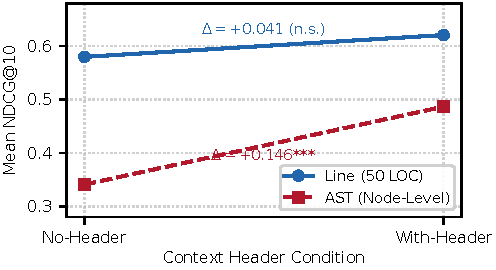
\includegraphics[width=0.72\columnwidth]{figs/fig1.pdf}
\caption{Interaction plot of context header sensitivity at reranking ($N=25$).}
\label{fig:interaction_plot}
\end{figure}

\begin{table}[t]
\caption{Hypothesis tests on NDCG@10 at reranking tier ($N=25$).}
\label{tab:statistical_hypothesis_tests}
\centering
\resizebox{\columnwidth}{!}{%
\begin{threeparttable}
\begin{tabular}{@{}llccc@{}}
\toprule
ID & Contrast ($A - B$) & $\Delta$ [95\% CI] & W/L/T & $p_{\mathrm{Holm}}$ \\
\midrule
\multicolumn{5}{@{}l}{\emph{Confirmatory family (step-down Holm, $\alpha = 0.05$)}} \\
Comp 1 & \astH\ vs. \lineN & $-0.093$ $[-0.164, -0.023]$ & 7/18/0 & $0.0438^{*}$ \\
Comp 2 & \astN\ vs. \lineN & $-0.239$ $[-0.292, -0.185]$ & 2/23/0 & $<0.001^{***}$ \\
Comp 3 & \astH\ vs. \astN & $+0.146$ $[+0.086, +0.207]$ & 23/2/0 & $<0.001^{***}$ \\
Comp 4 & \lineH\ vs. \lineN & $+0.041$ $[-0.012, +0.093]$ & 15/10/0 & $0.2411$ \\
\midrule
\multicolumn{5}{@{}l}{\emph{Exploratory (outside the Holm family)}} \\
Comp 5 & \astH\ vs. \lineH & $-0.134$ $[-0.199, -0.070]$ & 5/20/0 & $0.0003^{\dagger}$ \\
\bottomrule
\end{tabular}
\begin{tablenotes}\scriptsize
\item[] W/L/T: queries where $A$ wins, loses, or ties against $B$. Significance follows $p_{\mathrm{Holm}}$ (*~$<0.05$, **~$<0.01$, ***~$<0.001$). $^{\dagger}$~Unadjusted $p$ (exploratory).
\end{tablenotes}
\end{threeparttable}%
}
\end{table}


\textbf{RQ1 (Context Headers):} Prepending headers yields a large, significant gain for AST chunks (\textbf{Comp 3}: $\Delta = +0.146$, 95\% CI $[+0.086, +0.207]$, $p_{\mathrm{Holm}} = 0.0001$, $W = 24.0$; AST+H wins 23/25 JDs). In contrast, prepending headers to line windows yields a minor, non-significant gain (\textbf{Comp 4}: $\Delta = +0.041$, 95\% CI [$-0.012$, $+0.093$], $p_{\mathrm{Holm}} = 0.2411$, $W = 118.0$; 15 wins vs. 10 losses). As shown in Fig.~\ref{fig:interaction_plot}, headers act as vital anchors for fine-grained AST chunks while providing diminishing returns for 50-line windows.

\textbf{RQ2 (AST vs. Line):} Simple line windows without headers significantly outperform AST chunks with headers (\textbf{Comp 1}: $\Delta = -0.093$, 95\% CI [$-0.164$, $-0.023$], $p_{\mathrm{Holm}} = 0.0438$, $W = 78.0$; Line wins 18 vs. AST wins 7). Without headers, line windows strongly outperform AST chunks (\textbf{Comp 2}: $\Delta = -0.239$, 95\% CI [$-0.292$, $-0.185$], $p_{\mathrm{Holm}} < 0.001$, $W = 3.0$; Line wins 23/25). In the exploratory contrast with headers (\textbf{Comp 5}), line windows remain significantly superior ($\Delta = -0.134$, 95\% CI [$-0.199$, $-0.070$], $p_{\mathrm{raw}} = 0.0003$, $W = 36.0$; Line wins 20 vs. AST wins 5).

\subsection{Subgroups, Morphology Sensitivity, and Header Effects}
\label{sec:results:sensitivity}
\textbf{Subgroups \& Common Support:} Trends hold across languages: Java ($N=15$) yields Line+H $0.716$ vs. AST+H $0.583$ ($\Delta = -0.133$); React/TS ($N=10$) yields $0.478$ vs. $0.342$ ($\Delta = -0.136$). 
AST fallback is $0.0\%$ (0/438 chunks, 0/250 top-10 candidates). 
Evaluating on \textit{Common Support} (826/882 pairs where both strategies have candidate chunks, retaining 91.8\% of relevant evidence across all 25 queries) confirms that Line+H retains its statistically significant lead over AST+H ($0.600$ vs. $0.489$, $\Delta = +0.111$, $p_{\mathrm{Holm}} = 0.0036$, $W = 51.0$), while Line No-H dominates AST No-H ($0.535$ vs. $0.342$, $\Delta = +0.193$, $p_{\mathrm{Holm}} < 0.0001$, $W = 11.0$). 
Coverage accounts for only 17.3\% of the end-to-end gap ($+0.023$, $p = 0.0015$), demonstrating that Line superiority is driven primarily (82.7\%) by intrinsic contextual ranking.

\textbf{Window Overlap Sensitivity:} Suppressing intersecting 10-LOC overlapping windows from the same file in top-10 retrieval (26.4\% of Line top-10 slots involved in overlap [16.8\% redundant] vs. 0\% in AST) leaves deduplicated NDCG@10 intact: Line+H achieves $0.583$, Line No-H $0.574$, AST+H $0.482$, and AST No-H $0.341$. 
Line windows retain their significant lead (\textbf{Comp 5}: $\Delta = -0.101$, $p = 0.0013$; \textbf{Comp 1}: $\Delta = -0.092$, $p = 0.0236$), and the AST header boost remains large (\textbf{Comp 3}: $\Delta = +0.141$, $p < 0.001$).

\textbf{Qualitative Inspection of Header Lift:} Inspecting rank trajectories illustrates how headers ground isolated chunks. 
For \texttt{JD\_JAVA\_01} (\textit{"Spring Security \& JWT"}), the authenticated profile endpoint in \texttt{AccountController.java} (lines 39--64, \texttt{me()}, annotated \texttt{@SecurityRequirement}) rises from Rank~6 without header to Rank~1 with header (human relevance 2). 
For \texttt{JD\_REACT\_01} (\textit{"React Admin Dashboard \& RBAC"}), an administrative control panel in \texttt{Admin/index.tsx} (lines 544--613) jumps from Rank~13 to Rank~1 with header (relevance 2).

\section{Discussion and Threats to Validity}
\label{sec:discussion}

\subsection{Underlying Mechanisms and Scope}
In our setting, node-level AST extraction (without sibling merging as in \castname~\cite{zhang2025cast}) did not surpass sliding windows in requirement evidence retrieval. 
Three mechanisms may explain this; we did not test them directly: 
(1)~\textit{Information density and token budget}: 50-line windows (mean 41.0 LOC, 390.8 tokens) capture surrounding declarations, annotations, and helper calls, providing richer co-occurrence signals than isolated AST nodes (mean 26.7 LOC, 250.8 tokens). This token gap is expected from single-node extraction; without sibling merging, fine-grained AST slicing sacrifices contextual density. 
(2)~\textit{Contextual compensation}: headers inject architectural namespace, aiding cross-encoders to match requirement keywords against file and class names. Notably, AST headers carry more metadata (class and method cues), yet line windows remain superior. 
(3)~\textit{Query granularity}: composite JD queries (5--8 skills) may favor broader 50-LOC windows encompassing co-occurring functions over individual nodes.

\subsection{Threats to Validity}
\textbf{Internal Validity:} \textit{Pooling and blinding.} Mitigated by pooling all 12 systems at top-5 (so top-5 is fully judged by construction) and dual annotation with annotators blinded to system, header condition, rank, and score ($\kappa_w = 0.9822$; dual author annotation may carry expectation bias). \textit{Coverage and overlap.} Confounds from AST line coverage (69.0\% lines; median 16 vs. 50 LOC) and window overlap (26.4\% of Line top-10 slots involved in overlap [16.8\% redundant], vs. 0\% in AST No-Header and 0.8\% in AST+Header due to nested units) were audited: common-support evaluation ($N=826$ shared pairs) shows Line retains its lead ($\Delta = -0.111, p_{\mathrm{Holm}} = 0.0036$), and deduplication preserves ranking. \textit{Truncation and unjudged bias.} The reranker truncates at 512 tokens (28.6\% line vs. 15.8\% AST chunks exceed this). Pooling depth (5) is smaller than evaluation depth (10); unjudged items at ranks 6--10 receive zero gain. Because Judged@10 varies across systems (0.560--0.752; 0.660--0.736 at reranking, lowest for AST+Header), this bias is not uniform, though bpref yields identical condition rankings. \textit{Header asymmetry.} The two headers carry different metadata amounts (File and Lines for line windows; File, Class, Method, Lines for AST chunks), confounding the header effect with richness. \textit{Parser configuration.} Grammars were extended before final pooling; no judgments were collected with earlier parsers.
\textbf{Statistical Conclusion Validity:} With $N = 25$ queries, 80\% power requires paired differences of at least $\Delta \approx 0.08$--$0.13$ (the minimum detectable effect, MDE), given observed standard deviations $\sigma_d \in [0.137, 0.184]$ and $\alpha \in [0.0125, 0.05]$; non-significant small differences (e.g., Comp 4, $\Delta = +0.041$) indicate absence of evidence rather than equivalence.
\textbf{Construct Validity:} Requirements were extracted via \texttt{gemini-2.5-flash} (spot-checked by authors across the 25 JDs) to reflect authentic expectations. Curating core architectural modules yields cleaner candidate density than whole-repository search, though both strategies share the same files. Relevance was judged on a 3-point ordinal graded-relevance scale with task-specific definitions (Section~\ref{sec:approach:pooling}). 
\textbf{External Validity:} Evaluated on Java Spring Boot and React/TypeScript with BGE-M3 and BGE-Reranker-Base; caution is warranted when generalizing to dynamically typed languages or distributed architectures.

\section{Research Plan and Roadmap}
\label{sec:plan}

Table~\ref{tab:roadmap} outlines planned phases for RQ3 and RQ4: corpus expansion across four languages (Java, TypeScript, Python, Go; \textbf{P1}), graph-enriched headers via precomputed SCIP/LSIF code-index formats (\textbf{P2}), and developer verification studies seeking ethics approval (\textbf{P3}).

\begin{table}[t]
\caption{Research Roadmap and Milestones}
\label{tab:roadmap}
\centering\scriptsize
\setlength{\tabcolsep}{2pt}
\renewcommand{\arraystretch}{0.76}
\begin{threeparttable}
\begin{tabular}{@{}l>{\raggedright\arraybackslash}p{0.80in}>{\raggedright\arraybackslash}p{1.00in}>{\raggedright\arraybackslash}p{1.04in}@{}}
\toprule
Phase & Objective & Target Data & Analysis Method \\
\midrule
\textbf{P1} & Corpus Expansion (RQ3) & 100 repos (Java, TS, Py, Go); 50 JDs/issues & Factorial; mixed-effects models \\
\textbf{P2} & Graph Headers (RQ3) & Call-graphs \& imports vs. path headers & Paired Wilcoxon-Holm; ablations \\
\textbf{P3} & Human Study (RQ4) & $N=20$ software developers & Accuracy, inspection time, confidence \\
\bottomrule
\end{tabular}
\end{threeparttable}
\vspace{-6pt}
\end{table}

\section{Conclusion}
\label{sec:conclusion}
In this ERA paper, we presented a controlled $2 \times 2$ factorial evaluation crossing chunking strategy with hierarchical context headers across 40 repositories. 
At reranking, line-window chunking with headers achieved the highest performance ($\text{NDCG@10} = 0.621$), significantly outperforming AST chunks with headers ($\Delta = -0.134$, $p = 0.0003$). 
While context headers provide an essential boost for AST chunks ($\Delta = +0.146$, $p_{\mathrm{Holm}} = 0.0001$), line windows without headers significantly outperform AST chunks with headers ($\Delta = -0.093$, $p_{\mathrm{Holm}} = 0.0438$), and strongly outperform AST chunks without headers ($\Delta = -0.239$, $p_{\mathrm{Holm}} < 0.001$). 
Following parser grammar expansions, the AST fallback rate was $0.0\%$, confirming that node-level AST extraction without sibling merging does not surpass sliding windows in requirement evidence retrieval. 
We pose three open questions for the community:
(1)~\textit{Can graph-enriched headers bridge the information gap for fine-grained AST chunks?} 
(2)~\textit{How should code-RAG benchmarks weigh syntactic integrity against contextual information density?} 
(3)~\textit{How can requirement evidence retrieval best assist practitioners in verifying codebase capabilities?}

\section*{Data Availability}
The replication package (corpus code, frozen queries, Tree-sitter parsers, 882 blinded human-labeled pairs, adjudication records, and benchmark scripts) is available at: \url{https://anonymous.4open.science/r/ast-rag-replication-2027-82C5/}.

% \section*{Acknowledgments}
% Omitted for double-anonymous review. Generative AI tools (Google Antigravity, Anthropic Claude, Gemini) assisted in drafting text, code refactoring, and statistical script generation; all outputs were verified by the authors. Relevance labels were produced entirely by human annotators without AI intervention.


\bibliographystyle{IEEEtran}
\bibliography{refs}

\end{document}
